
\chapter{Method 2: Tri-dexel}
\label{ch:tri_dexel}

The second discussed method to extract a triangulated surface from the VML's data model is based on a tri-dexel representation, \cf section \ref{sec:surface_representations}.
As observed with the previously shown method in chapter \ref{ch:direct_intersection}, reconstructing a surface directly form the many intersecting triangles stored in the VML's grid is computationally expensive, highly numerically unstable and prone to errors.
A more robust approach is desirable, which is able to always successfully reconstruct a surface with good quality.
This reconstruction should succeed independently of the complexity of the maintained geometry.
As a trade-off for this robustness, the approach may sacrifice surface exactness and filigree features.
Dexel-based representations fit this purpose nicely.
They provide a good abstraction of a machined workpiece with rich semantics.
The used grid resolution supplies an easy to configure level of detail and steering parameter between representation quality and memory/CPU demands.
Creating dexel-based representations from the VML's data model is achieved using an adaption of the already implemented, well-working and robust raycasting subsystem used for visualization, \cf section \ref{sec:raycasting}.
To achieve a good portrayal independently of the workpiece's orientation, three axis-aligned dexel images will be generated, thus creating a tri-dexel representation.
For converting such a tri-dexel model into a final triangle mesh, various algorithms are found in literature.
An excellent example is Ren \etal's "Feature Conservation and Conversion of Tri-dexel Volumetric Models to Polyhedral Surface Models for Product Prototyping" \cite{tridexel_reconstruction}.
Their approach form the idea and foundation of the implementation presented in this chapter.


\section{Concept}
\label{sec:tri_dexel_concept}

Firstly, a tri-dexel representation of the VML's data model has to be obtained.
Dexel images, in general, are created by sampling the workpiece's surface along parallel lines.
This sampling process is already implemented in the raycasting subsystem as part of the visualization.
However, when sampling dexels, a ray must not stop at the first surface intersection, but continue through the whole data model and collect all intersections along its path.
At each intersection, the intersection depth, \ie distance from the ray's origin, and the surface normal of the intersected triangle is recorded as a dexel node.
From the dexel's origin and a node's depth the intersection point can be calculated.
The raycast itself is performed with axis-parallel rays starting at equidistant origins from three sides of the VML's data model, thus creating three dexel images.
Combining these dexel images creates a uniform regular grid, the tri-dexel grid.
Figure \ref{fig:cylinder_head_dexel} shows the cylinder head scene with a low-resolution dexel image and the final reconstruction.

\begin{figure}
	\centering
	\begin{subfigure}[t]{0.3\textwidth}
		\centering
		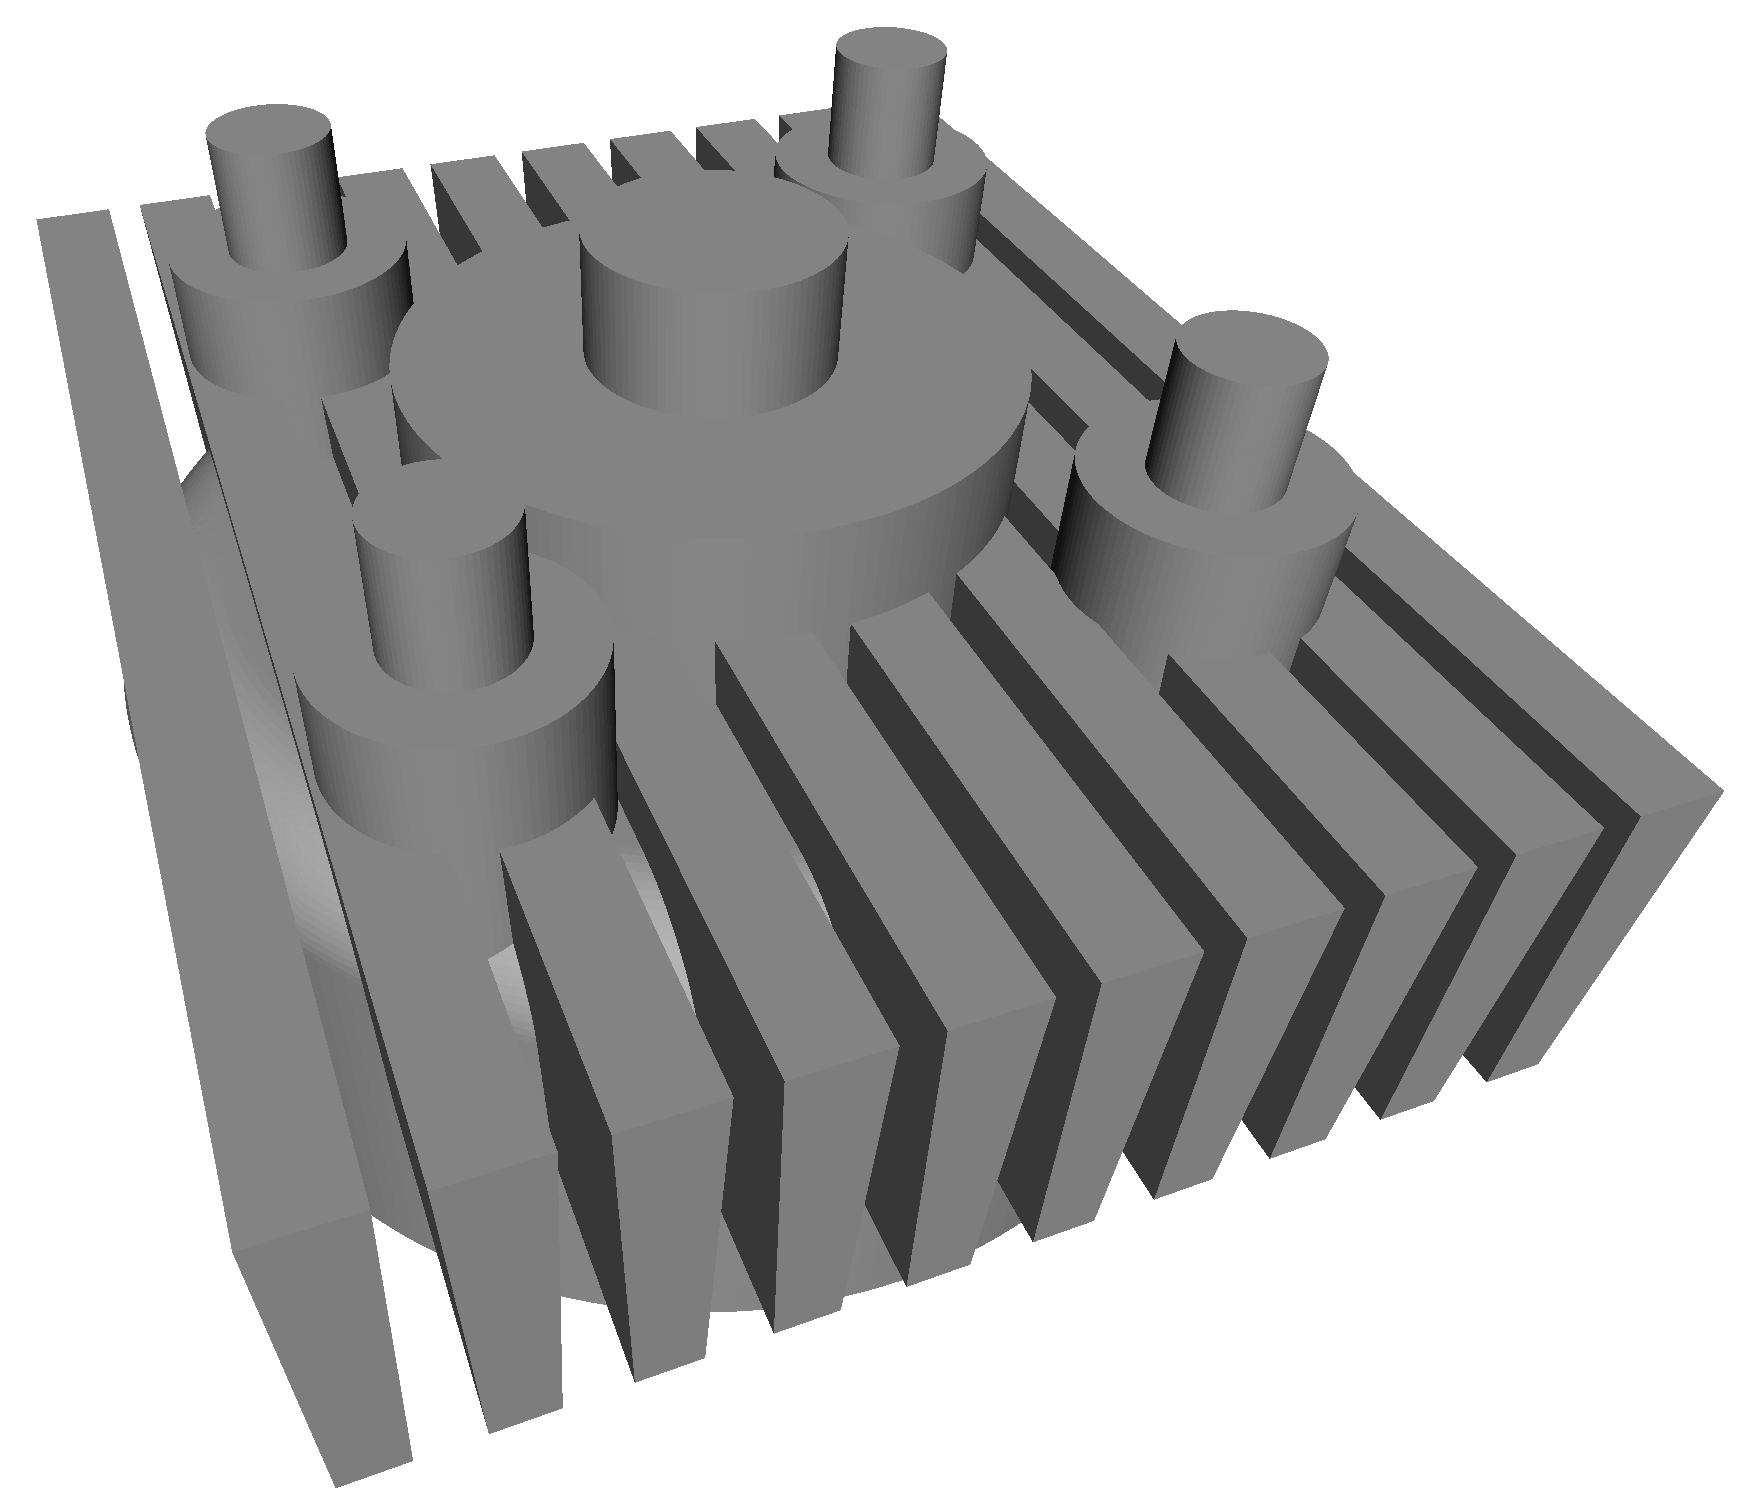
\includegraphics[width=\textwidth]{images/cylinder_head_stock_and_svs}
		\caption{Stock and SVs}
		\label{fig:cylinder_head_stock_sv}
	\end{subfigure}
	\begin{subfigure}[t]{0.3\textwidth}
		\centering
		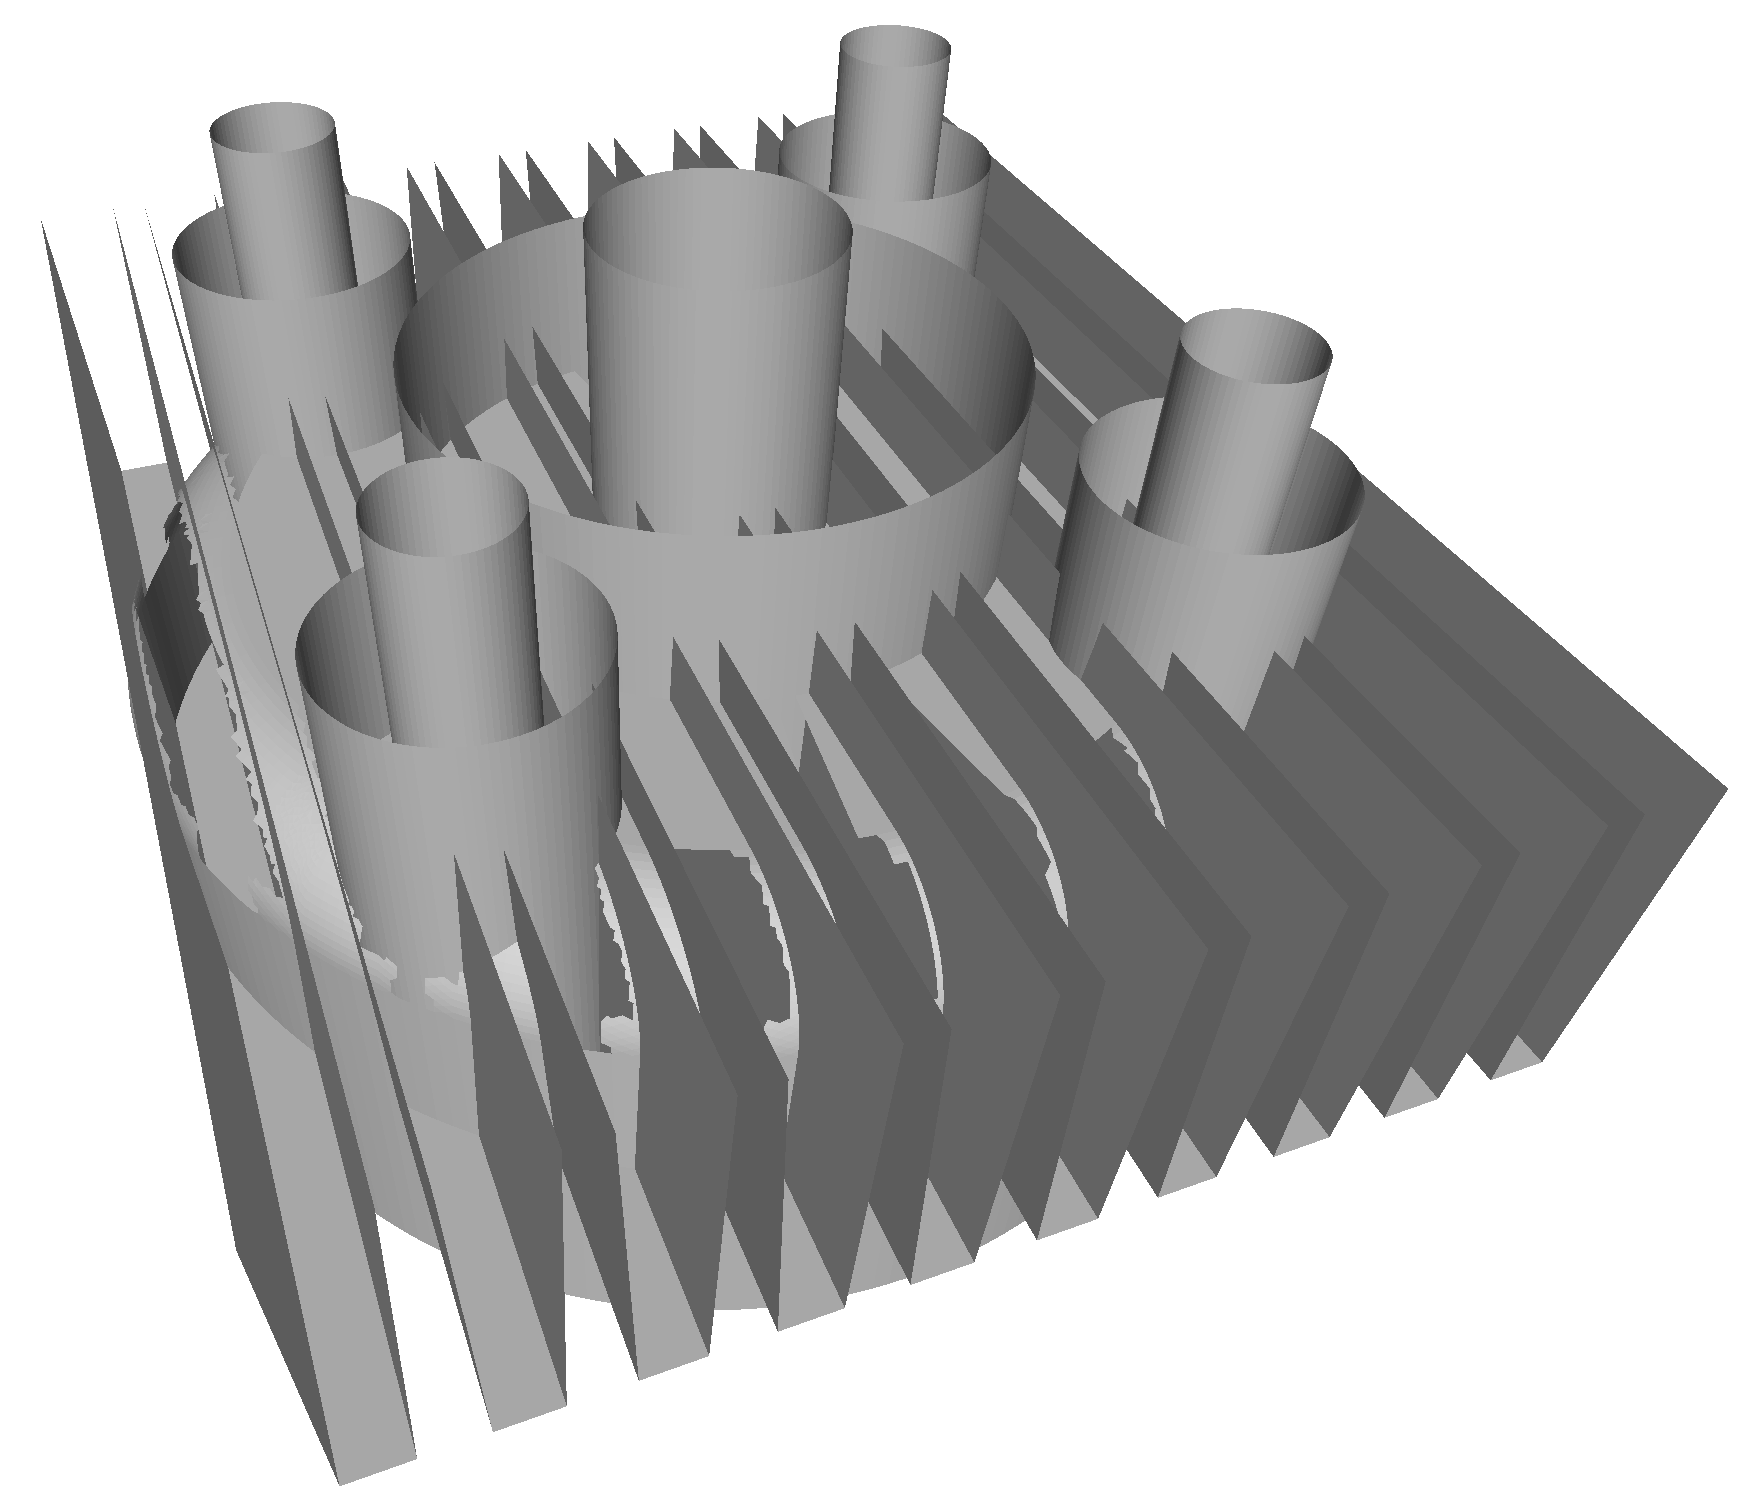
\includegraphics[width=\textwidth]{images/cylinder_head_vml}
		\caption{VML}
		\label{fig:cylinder_head_classified}
	\end{subfigure}
	\begin{subfigure}[t]{0.3\textwidth}
		\centering
		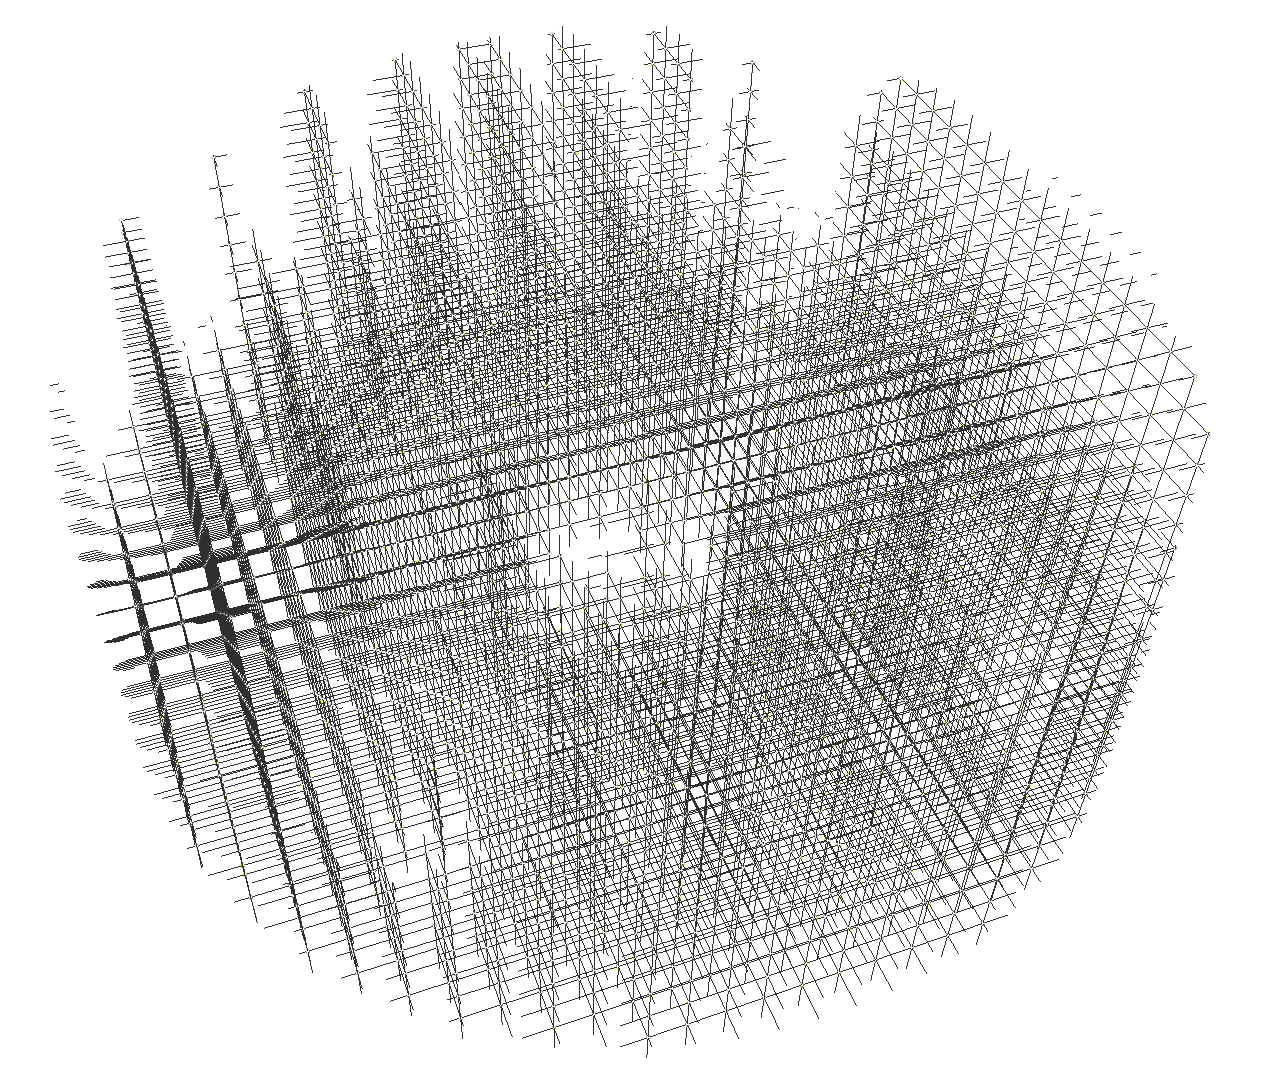
\includegraphics[width=\textwidth]{images/cylinder_head_dexel_image}
		\caption{Tri-dexel image}
		\label{fig:cylinder_head_dexel_image}
	\end{subfigure}
	\begin{subfigure}[t]{0.3\textwidth}
		\centering
		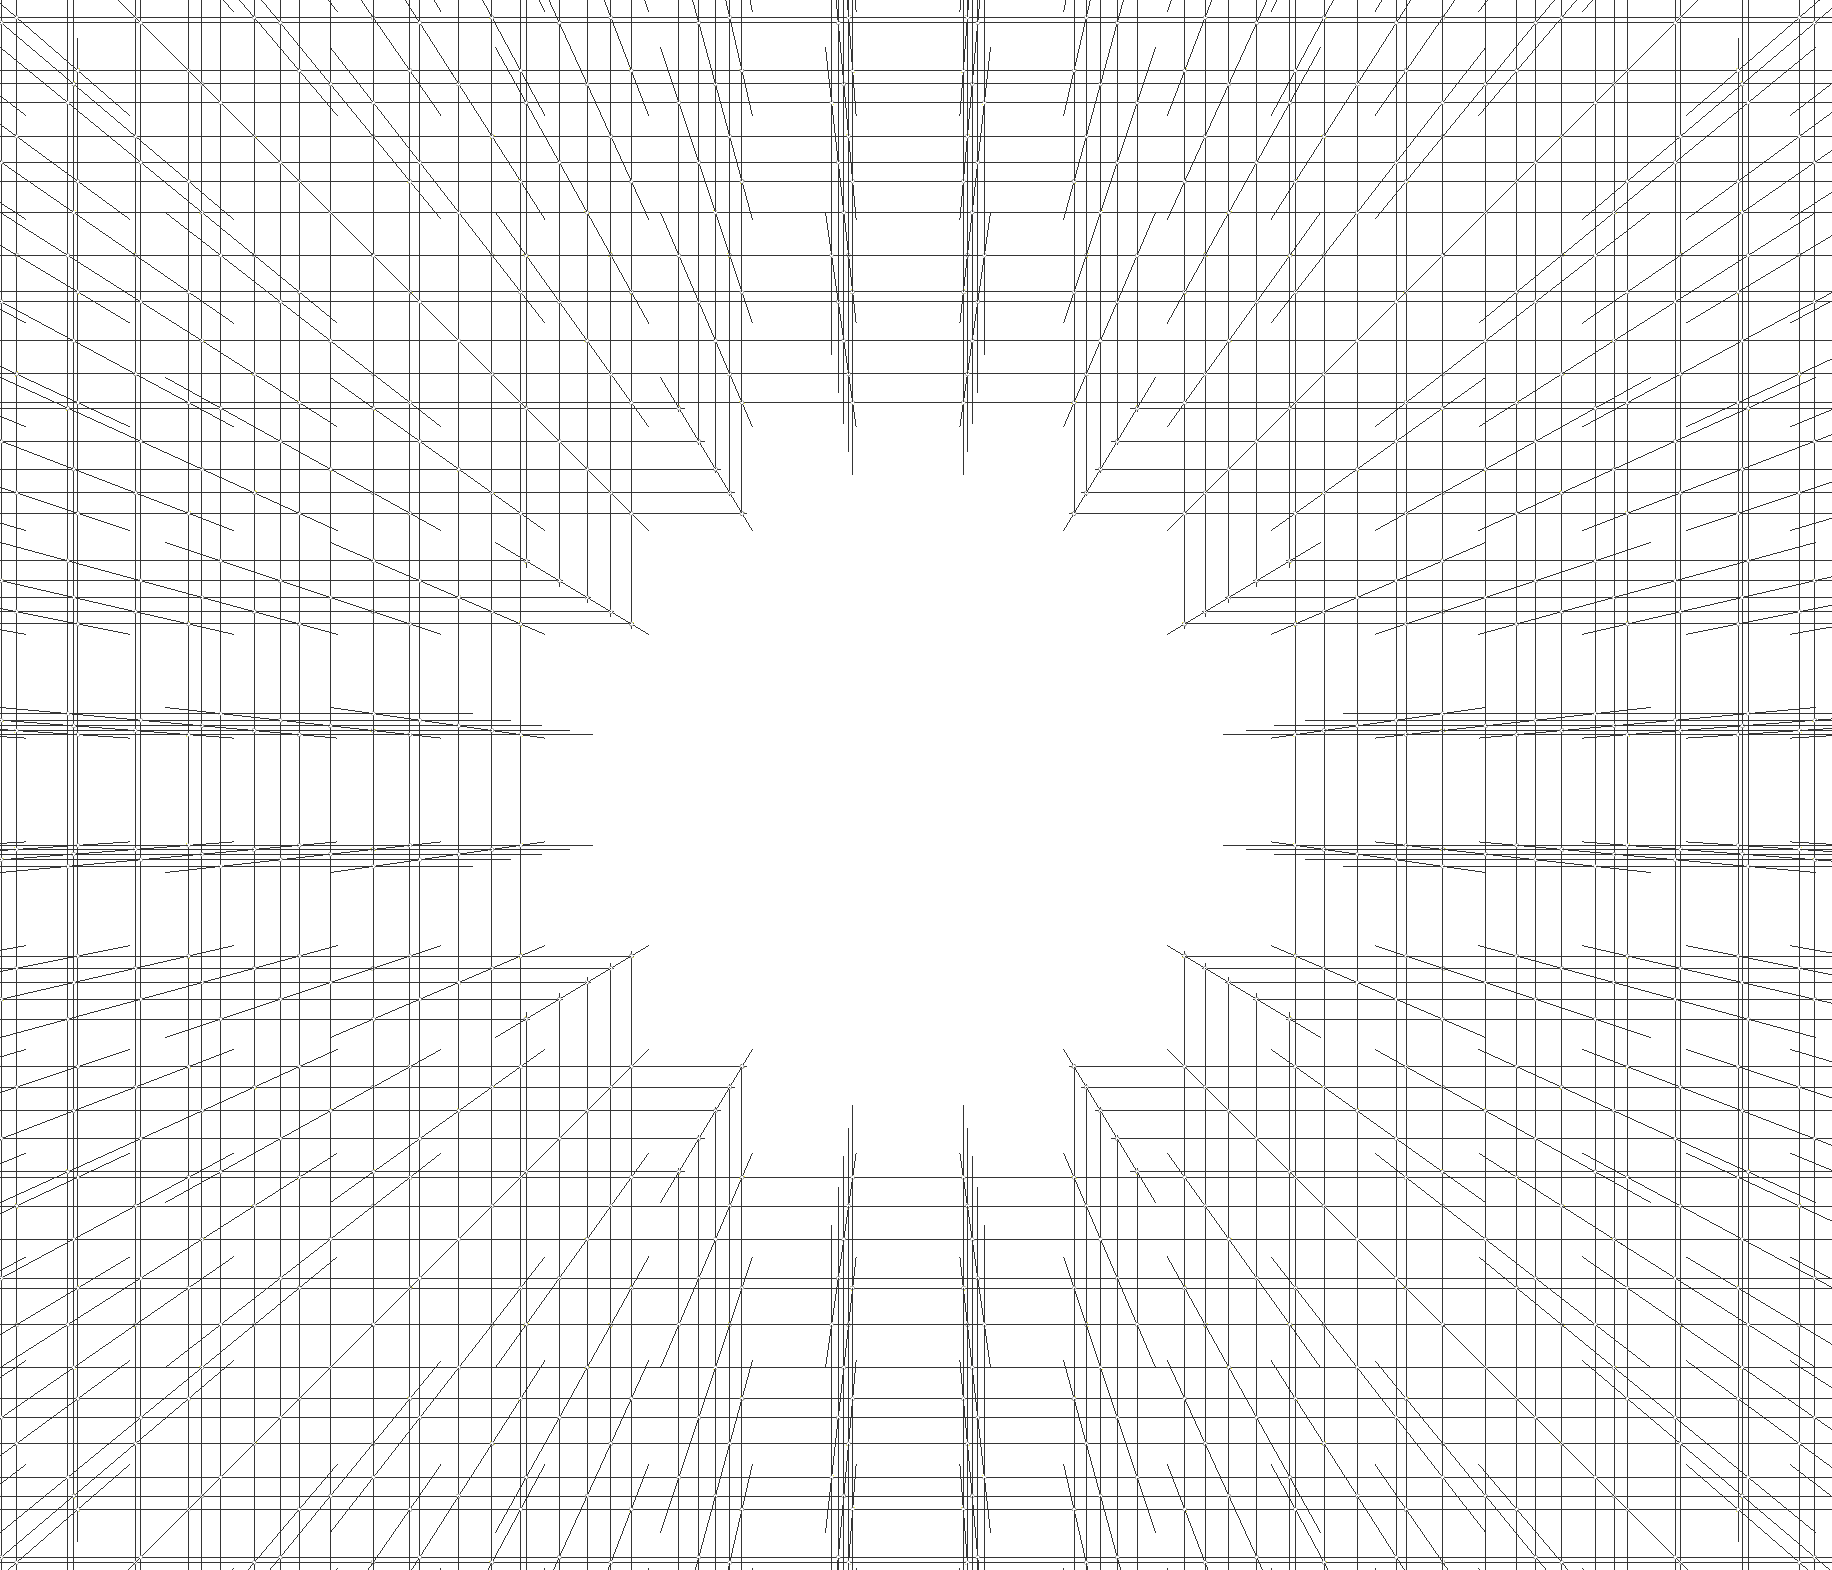
\includegraphics[width=\textwidth]{images/cylinder_head_dexel_image_center}
		\caption{Tri-dexel image center}
		\label{fig:cylinder_head_dexel_image_center}
	\end{subfigure}
	\begin{subfigure}[t]{0.3\textwidth}
		\centering
		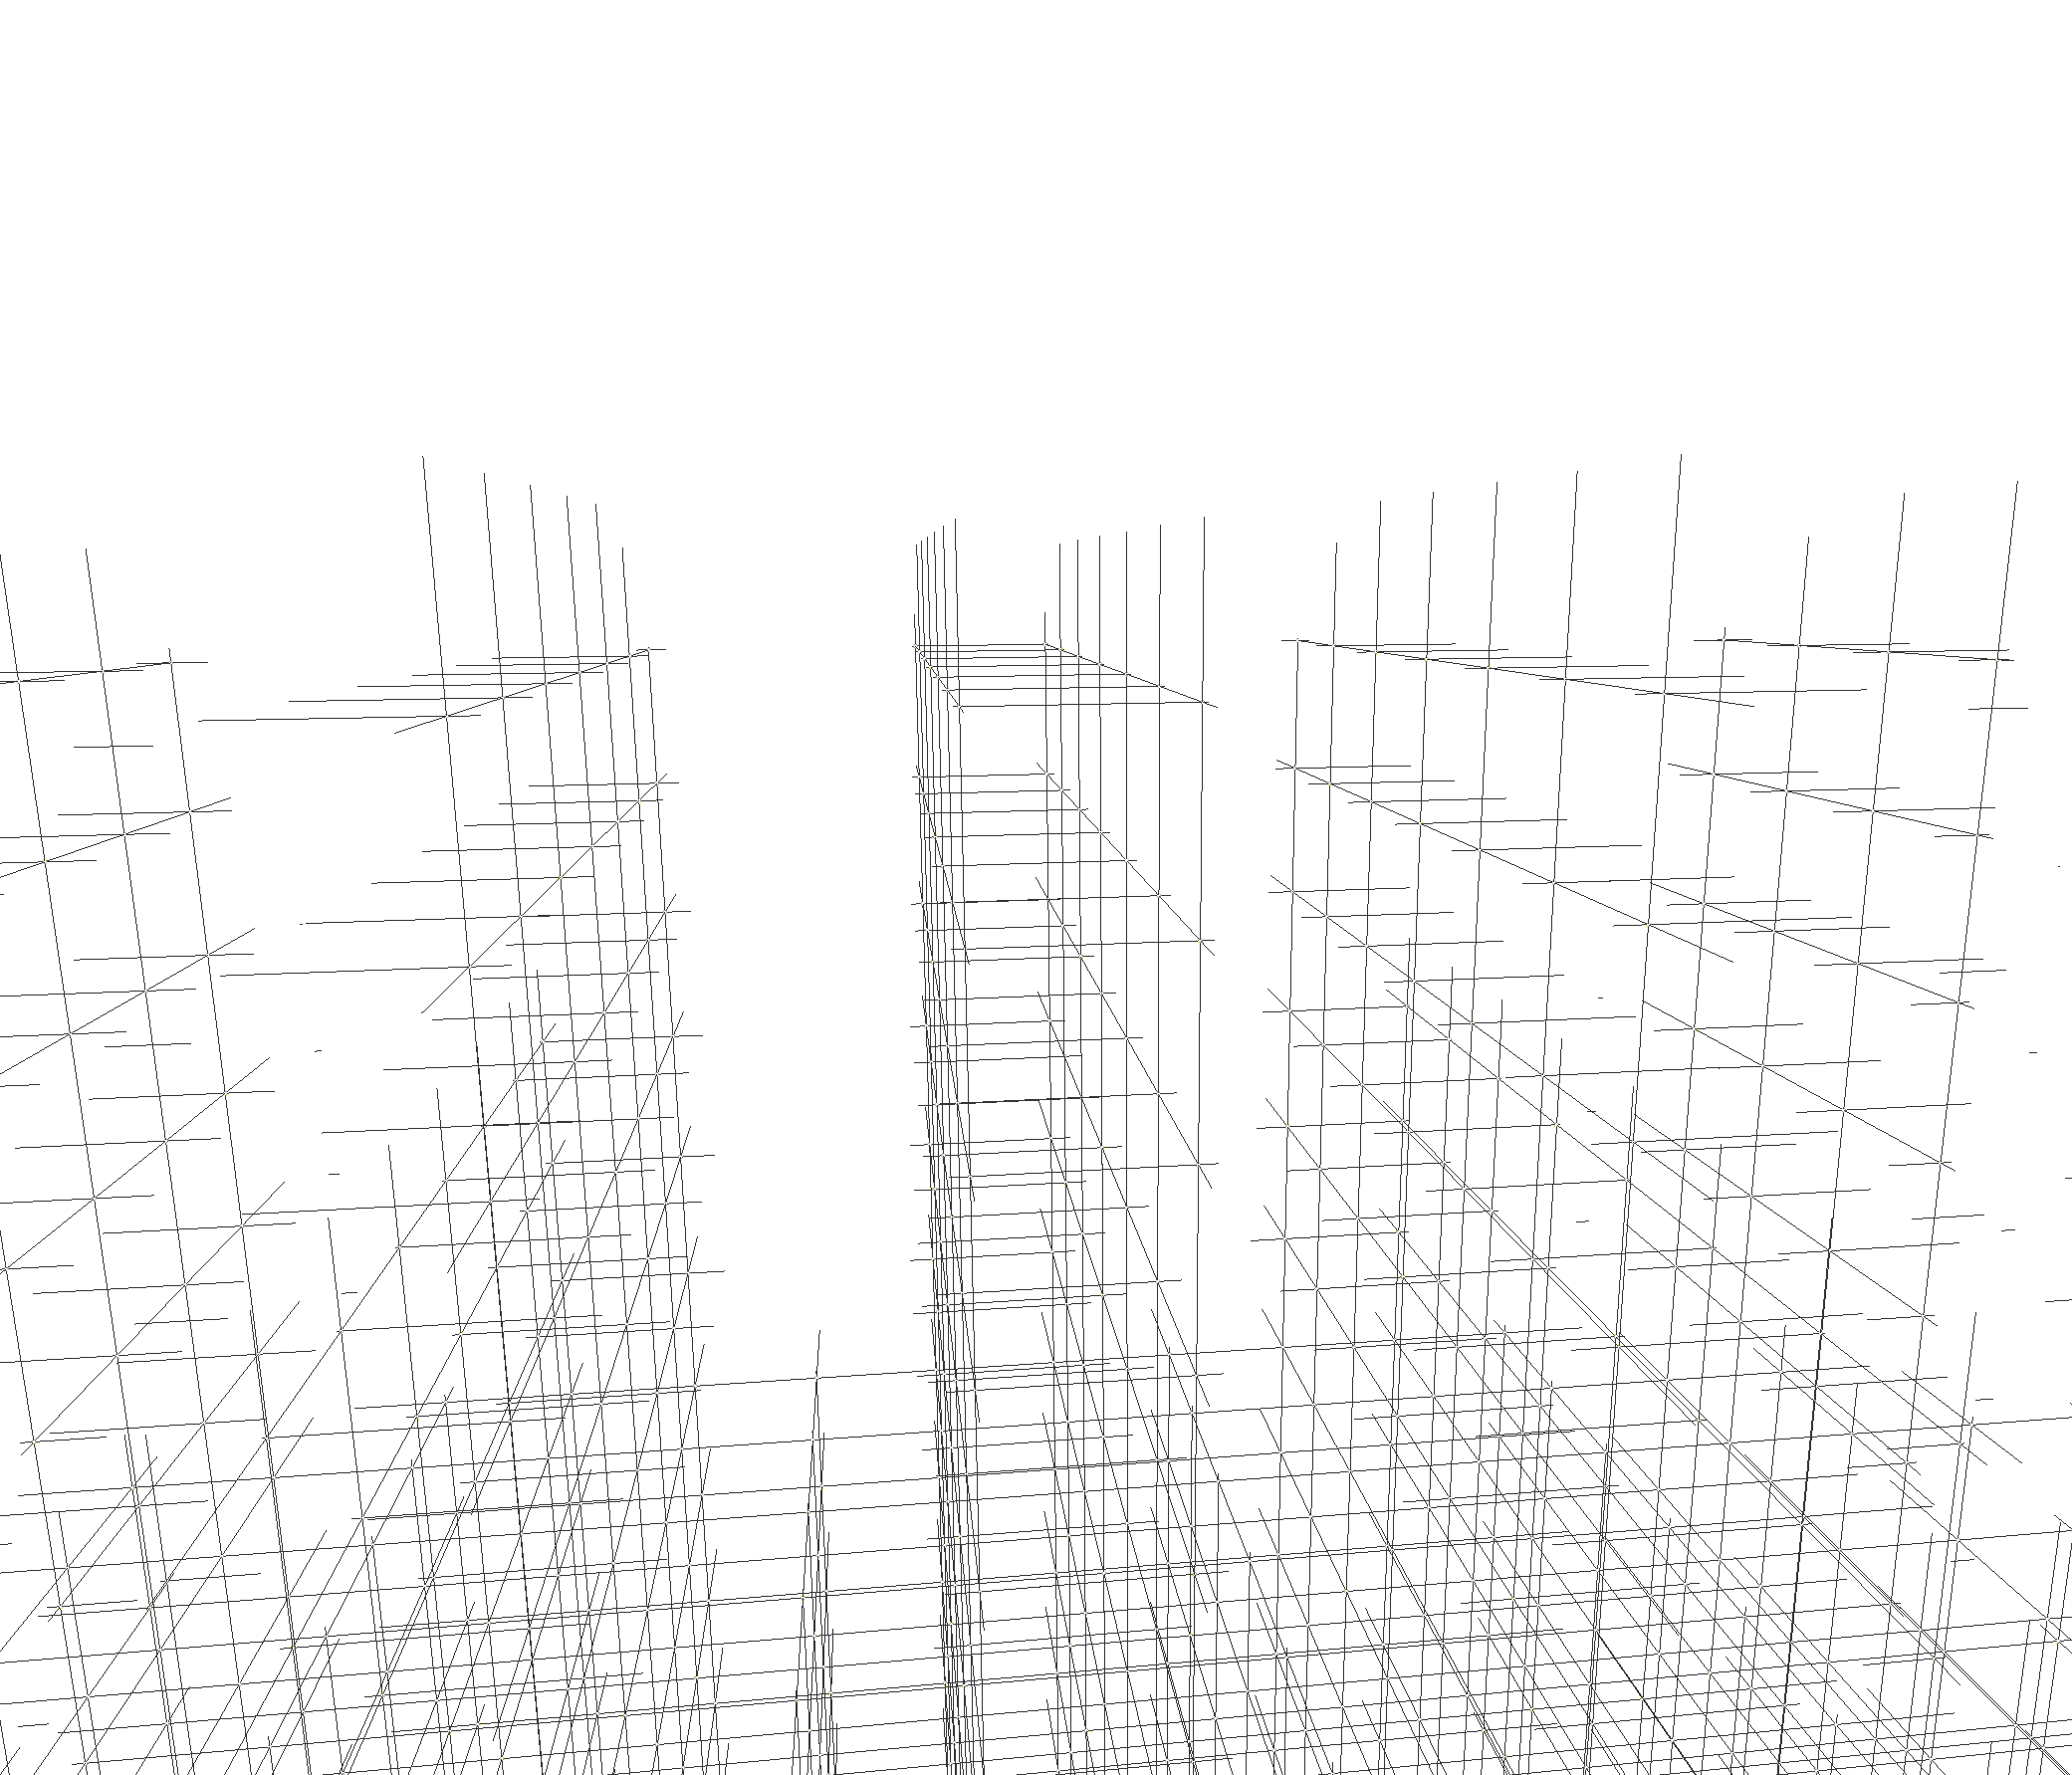
\includegraphics[width=\textwidth]{images/cylinder_head_dexel_image_fins}
		\caption{Tri-dexel image fins}
		\label{fig:cylinder_head_dexel_image_fins}
	\end{subfigure}
	\begin{subfigure}[t]{0.3\textwidth}
		\centering
		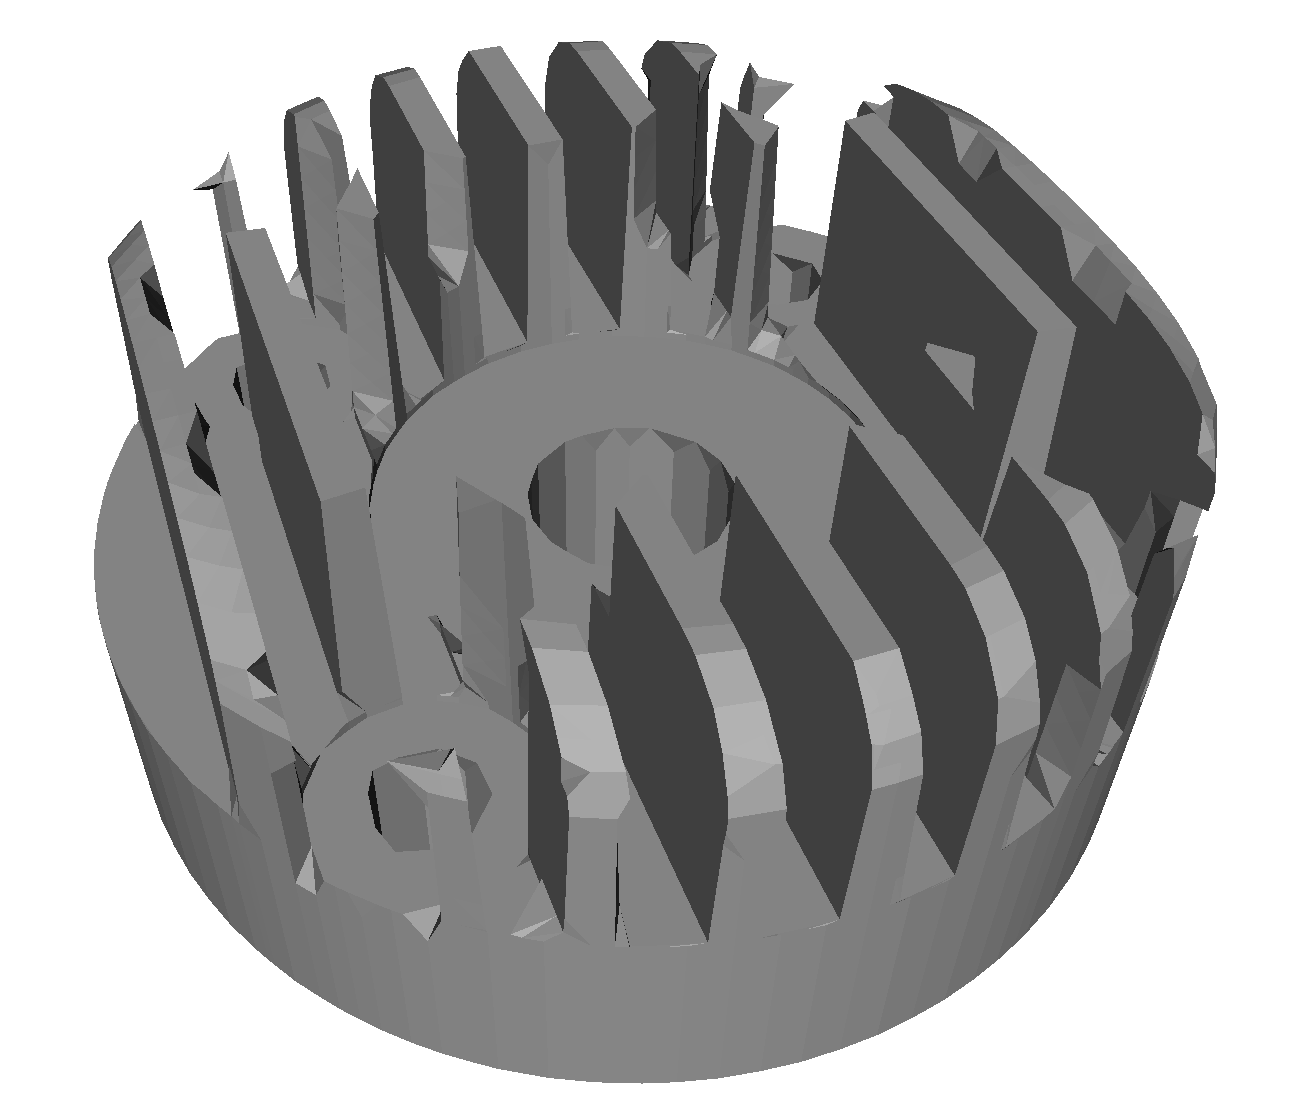
\includegraphics[width=\textwidth]{images/cylinder_head_reconstructed}
		\caption{Result}
		\label{fig:cylinder_head_reconstructed}
	\end{subfigure}
	\caption{
		Tri-dexel based surface reconstruction from the VML's data model of a cylinder head.
		Figure \ref{fig:cylinder_head_stock_sv} shows the stock and a few swept volumes creating the fins and drillings.
		Figure \ref{fig:cylinder_head_classified} shows the classification result after these solids have been mapped into the VML's regular grid.
		The removed triangles are clearly visible, especially at the swept volumes.
		By using a raycast of axis parallel rays along all three coordinate system axes a tri-dexel representation is created as shown in figure \ref{fig:cylinder_head_dexel_image}.
		The resolution of the grid spawning the rays is 30 along the longest dimension.
		Figure \ref{fig:cylinder_head_dexel_image_center} and \ref{fig:cylinder_head_dexel_image_fins} show details of the tri-dexel image.
		The former views the drilling at the center from above and the latter views the cylinder head's fins from the center.
		Finally, the reconstructed surface is shown in figure \ref{fig:cylinder_head_reconstructed}.
		Note the imperfections at the fin's edges and bases.
	}
	\label{fig:cylinder_head_dexel}
\end{figure}

Secondly, the tri-dexel representation is converted into a triangle mesh.
This procedure is mostly based on the paper already mentioned during the introduction \cite{tridexel_reconstruction}.
Each intersection point of three orthogonal dexels from the tri-dexel grid forms a grid point.
If a grid point lies within a dexel segment on any of these dexels, it is said to be occupied, \ie lies within the workpiece's volume.
8 grid points and their 12 connecting edges along with their dexel segments are grouped into cells of the grid.
Each grid cell is then processed independently.
Figure \ref{fig:tri_dexel_cell} shows the structure of a tri-dexel cell.
%
\begin{figure}
	\centering
	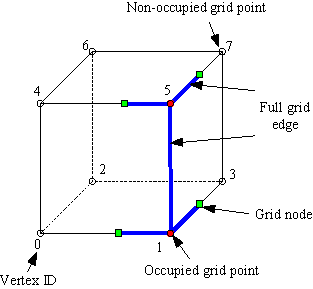
\includegraphics[width=0.5\textwidth]{images/tri_dexel_cell}
	\caption{
		A cell of a tri-dexel grid \cite{tridexel_reconstruction}.
		Occupied grid points are drawn in red, dexel nodes in green, dexel segments in blue.
		Each grid point is referenced using a number between 0 and 7 and has a list of neighboring grid points in counter-clockwise order, \cf left table.
	}
	\label{fig:tri_dexel_cell}
\end{figure}
%
Before a cell can be triangulated, a few consistency checks and corrections are applied to the cell.
This process is called regularization and ensures a successful triangulation into a water-tight mesh.
After ensuring the consistency of a cell, it can be triangulated.
For this purpose, a depth-first search process is iteratively started at non-occupied grid points of the cell to discover boundary loops.
Basically, the found loops can be triangulated right away to obtain a water tight mesh.
However, the quality of the triangulation can be further enhanced by taking normal information at the dexel nodes into account.
This is especially necessary to reconstruct features of the model.
This optional feature reconstruction pass is run on the loops found in the previous step and may create additional vertices.

\section{Implementation}
\label{sec:tri_dexel_implementation}

In order to run the tri-dexel surface reconstruction, the user must supply a resolution as parameter.
This resolution determines the size of the raycasted dexel images as well as the resulting tri-dexel grid.
For esthetic reasons, the specified resolution is only used for the longest dimension of the workpiece.
The resolution along the other dimensions is usually smaller in order to make the cells more cubic, although the implementation does not require cubic cells.

cutting dexels

\begin{algorithm}
	\centering
	\begin{algorithmic}[1]
		\Function{TriDexel}{$\var{grid}, \var{resolution}$}
		\EndFunction
	\end{algorithmic}
	\caption{
		Abstract workflow of the surface reconstruction using a tri-dexel approach.
	}
	\label{alg:direct_intersection}
\end{algorithm}


\subsection{Raycast}
\label{sec:tri_dexel_raycast}



\subsection{Dexel image generation}
\label{sec:tri_dexel_dexel_image_generation}



\subsection{Regularization}
\label{sec:tri_dexel_regularization}



\subsection{Triangulation}
\label{sec:tri_dexel_triangulation}

For this purpose, a depth-first search process is iteratively started at non-occupied grid points of the cell.
The search traverses the cell's edges and backtracks each time an occupied grid point and therefore a grid edge containing a dexel node is found.
The list of visited grid edges containing dexel nodes, in the order they where visited, forms a boundary loop.
A cell might contain multiple boundary loops, found when starting at different, non-occupied grid points.

\subsection{Refinement and feature reconstruction}
\label{sec:tri_dexel_refinement}

This optional feature reconstruction pass is run on the loops found in the previous step.
Using the normals of each pair of adjacent dexel nodes of the loop, an additional intermediate/feature point may be created.
Using the normals of multiple nodes, a further apex vertex may be created per loop.
Finally, these enhanced loops are also triangulated.

\subsection{Subslicing *experimential*}
\label{sec:tri_dexel_subslicing}



\subsection{Parallelization}
\label{sec:tri_dexel_parallelization}



\section{Results}
\label{sec:tri_dexel_results}


